\chapter{规划测量：精密度、准确度与效度}
\chapterauthors{Steven R. Cummings、Thomas B. Newman、Alison J. Huang}
% Chinese reconstructions of source PDF figures 3.1--3.4.
\newcommand{\chfouroverview}{%
\begin{tikzpicture}[x=1cm,y=1cm,font=\small,>=Stealth,
 panel/.style={draw=dcrblue!65,line width=.7pt,fill=white,align=center,text width=3cm},
 base/.style={draw=dcrred,fill=white,line width=.8pt,minimum width=3.15cm,minimum height=.9cm,align=center}]
\foreach \x/\t/\a/\b in {0/研究问题/目标人群/目标现象,5/研究计划/预定样本/预定变量,10/实际研究/实际样本/实际测量}{
\node[panel,minimum height=2.5cm] (c\x) at (\x,0) {};
\node[fill=dcrblue!65,text=white,align=center,minimum width=3.15cm,minimum height=.7cm] at (\x,1.05) {\bfseries\t};
\node at (\x,.25) {\a};\node at (\x,-.65) {\b};}
\draw[->,line width=3pt,dcrblue!65] (1.6,-.65)--(3.4,-.65) node[midway,above,font=\small] {设计};
\draw[->,line width=3pt,dcrblue!65] (6.6,-.65)--(8.4,-.65) node[midway,above,font=\small] {实施};
\draw[red,line width=1.2pt] (-1.75,-1.05) rectangle (11.75,-.25);
\node[text=dcrgold,align=center] (choice) at (5,-2.2) {选择与误差\\影响……};
\node[text=gray,align=center] (ev) at (2,-3) {外部\\效度};
\node[text=gray,align=center] (iv) at (8,-3) {内部\\效度};
\node[base] (understand) at (0,-5) {现有认识};
\node[base] (conclusion) at (5,-5) {研究结论};
\node[base] (result) at (10,-5) {研究结果};
\draw[->,gray,thick] (choice)--(ev);\draw[->,gray,thick] (choice)--(iv);
\draw[->,gray,thick] (ev)--(2.5,-.7);\draw[->,gray,thick] (ev)--(understand);
\draw[->,gray,thick] (iv)--(7.5,-.7);\draw[->,gray,thick] (iv)--(11.85,-3);
\draw[->,gray,thick] (iv)--(conclusion);
\draw[->,line width=3pt,dcrred!75] (result.west)--(conclusion.east) node[midway,above,font=\small] {解释};
\draw[->,line width=3pt,dcrred!90] (conclusion.west)--(understand.east) node[midway,above,font=\small] {推断};
\draw[->,line width=2pt,dcrblue!70] (c10.east)--(12.3,0)--(12.3,-5)--(result.east) node[pos=.43,right,font=\small,text=black] {分析};
\draw[->,line width=2pt,dcrred!85] (understand.west)--(-2.3,-5)--(-2.3,0)--(c0.west) node[pos=.43,left,font=\small,text=black] {思考};
\end{tikzpicture}}

\sourcepage{79}
测量以能够进行统计分析的形式描述现象。研究的有效性，取决于研究中设计和实际测量的变量，在多大程度上代表所关注的现象（图 4.1）。例如，父母回忆的出生体重，能在多大程度上反映实际出生体重（1）？这些概念对所有类型的测量都重要，包括体格检查、实验室检查和问卷评分。
\par
\begin{figure}[htbp]\centering\resizebox{\linewidth}{!}{\chfouroverview}
\caption*{\textbf{图 4.1}\quad 本章关注红框中的事项：设计能够代表研究问题所关注现象的测量。}
\end{figure}\par
\sourcepage{80}
本章先讨论测量尺度的选择如何影响测量所含的信息，再介绍一个中心目标：通过设计相对精密（随机误差少）且无偏倚（系统误差少）的测量，尽可能提高检查的准确度，使根据测量推断所关注现象更为恰当。随后讨论在定性层面与准确度相近的效度。最后介绍临床及转化研究中其他值得考虑的问题，特别是保存样本以供日后测量的优点。

本章讨论既适用于预测变量和结局变量，也适用于研究中其余测量变量，即\term{协变量}（covariates）。某些协变量的方法可以沿用既往研究，不必详细规划；但主要预测因素、主要结局，以及可能的少数其他变量，几乎总需要特别关注，使测量符合本项研究的具体需求。

\section{测量尺度}
表 4.1 简要分类介绍测量尺度及所含信息。不同类型变量的信息量不同，因而影响研究效能、样本量要求及所能揭示的分布细节，这使分类很重要。
{\small\setlength{\tabcolsep}{3pt}
\begin{longtable}{L{20mm}L{37mm}L{28mm}L{35mm}L{25mm}}
\caption*{\textbf{表 4.1}\quad 测量尺度}\\
\toprule 测量类型 & 变量特征 & 例子 & 描述统计量 & 统计效能\\\midrule\endfirsthead
\toprule 测量类型 & 变量特征 & 例子 & 描述统计量 & 统计效能\\\midrule\endhead
\multicolumn{5}{c}{\textbf{分类变量}}\\
二分类 & 两个类别 & 生存状态（活着或死亡） & 计数、比例 & 低\\
无序分类 & 类别无顺序 & 性别认同；血型 & 同上 & 低\\
\sourcepage{81}有序分类 & 类别有顺序，但间距无法量化 & 疼痛程度（无、轻、中、重）；社会阶层 & 除上述外，可用中位数 & 中等\\\midrule
\multicolumn{5}{c}{\textbf{数值变量}}\\
连续 & 取值数无限 & 体重；血红蛋白水平 & 除上述外，可用均值、标准差 & 高\\
离散或计数\textsuperscript{a} & 取值数有限，通常为整数 & 妊娠次数；性伴侣数 & 取值少时同有序变量；取值多时同连续变量 & 可能取值多时较高，尤其均值接近中间时\\\bottomrule
\multicolumn{5}{L{150mm}}{\footnotesize\textsuperscript{a}计数变量是只能取非负整数（0、1、2、3、……）的离散变量。}\\
\end{longtable}}

\subsection{分类变量：二分类、无序分类与有序分类}
不适宜量化的现象，通过归入类别来测量。有两个可能取值（例如死亡或存活）的\term{分类变量}（categorical variables），称为\term{二分类变量}（dichotomous variables）。类别多于两个的多分类变量（polychotomous variables），还可按信息类型进一步划分。其中，\term{无序分类变量}（nominal variables）的类别没有顺序，例如 A 型血既不比 B 型血多，也不比它少。
\sourcepage{82}
这类变量常有明确的定性特征，因而容易测量。相反，\term{有序分类变量}（ordinal variables）有顺序，例如重度、中度和轻度疼痛。相较无序分类，它包含更多信息；但相邻类别间的差或比并非可量化、等距的，故信息仍少于数值变量。

\subsection{数值变量：连续与离散}
\term{数值变量}（numerical variables）可用表示“多少”的数字来量化。\term{连续变量}（continuous variable），例如血红蛋白水平，在理论上取值无限的尺度上表示数量，虽然测量方法实际只会产生其中一部分值。相反，\term{离散变量}（discrete variable）的取值可数，通常以正或负整数表达，例如大流行期间一个家庭居住人数的变化。如果离散变量在较多可能取值，例如六个或更多，分布得较好，统计分析时就可能近似连续变量；在设计测量时，也可视为相当。

\subsection{选择测量尺度}
一个好的通则是：能够选择时，连续变量优于分类变量，因为额外信息能够提高统计效率。例如，比较几种治疗的降压效果时，以 mm Hg 记录血压，可观察每个人变化的大小；只分为高血压或正常血压，则限制了评估。连续变量信息更多，因而效能更高，或者所需样本量更小（第 5、6 章）。

连续变量也更灵活，便于根据变量性质或关联形状拟合数据，尤其关系可能复杂时。例如，研究体重指数（body mass index，BMI）与死亡的关联，
\sourcepage{83}
就可能发现 U 形模式：BMI 过低或过高者死亡率均高于中间者（2），并可描述死亡率开始改变的阈值。研究低出生体重预测因素时，应记录实际出生体重，而非仅记录是否低于传统的 2500 g 界值。这样可保留多种分析选择，例如改变低出生体重界值、划分多个有序类别（如 $<1500$、1500～1999、2000～2499 及 $\geq2500$ g），或直接使用连续测量值。

同样，设计医疗满意度等有序尺度的问题时，若能选择类别数，通常可以从“非常同意”到“非常不同意”提供约六个类别。以后可以合并为同意与不同意两个类别，反过来却不可能。

疼痛或生活质量等许多特征，难以用类别或数字描述，但量化对回答重要问题不可缺少。生活质量标准问卷简明健康调查 SF-36（Short Form-36）就是一例：它为八个维度提供离散数值评分，包括身体、社会、情绪功能及总体健康感（3）。分类和测量如果设计得好，可以增进知识的客观性、减少偏倚，并使交流更详细。

\section{精密度}
变量的\term{精密度}（precision）是测量可以重复、每次都得到近似数值的程度。杠杆秤可以非常精密地测体重；而用闭眼双脚并拢站立的持续时间衡量平衡能力，则可能随观察者或测量时机而变化。精密度对研究效能影响很大。在给定样本量下，测量越精密，检验关于该测量的假设时统计效能越高（第 5 章）。
\sourcepage{84}
精密度也称可重复性、可靠性或一致性（reproducibility、reliability、consistency），取决于随机误差，即偶然变异；误差越大，测量越不精密。主要有三种随机误差来源。
\begin{itemize}
\item \textbf{观察者变异}（observer variability）源于观察者，例如访谈措辞或操作机械仪器的技能。
\item \textbf{仪器变异}（instrument variability）源于仪器，例如环境温度变化、试剂批次差别等。
\item \textbf{参与者变异}（participant variability）源于参与者特征中与研究变量无关、但影响测量的固有变异。例如，力量测量可能受一天中的时段、距离上次进食的时间或用力程度影响。
\end{itemize}

\subsection{评估精密度}
精密度可用重复测量的可重复性评估，比较同一人（观察者内）或不同人（观察者间）的测量，也可比较同一仪器内或仪器间的测量。连续变量通常用参与者内标准差，或\term{变异系数}（coefficient of variation，即参与者内标准差除以均值）表示。\footnote{每人测量一个连续变量两次时，可能会想用相关系数表示一致性。但相关系数对离群值非常敏感，更好的方法是 Bland–Altman 图（4），将两次测量的差值对两次均值作图。如果差值的绝对值随均值近似线性增加，变异系数就比参与者内标准差更适合概括变异。}分类变量常用一致百分比、组间相关系数（原文为 interclass correlation coefficient）及 kappa 统计量（4～6）。

\subsection{提高精密度的策略}
减少随机误差、提高精密度有五种方法（表 4.2）。
\begin{enumerate}
\item \textbf{测量方法标准化。}每项方案都应详细说明测量方法，包括书面说明配图或短视频，介绍如何准备环境与参与者、实施和记录测量、校准仪器等（附录 4A）。
\sourcepage{85}
这些材料是操作手册的一部分，对大多数研究不可缺少。即使只有一名观察者，每项测量的书面具体指南，也有助于保证她在整个研究期间操作一致，并为发表结果时描述方法提供依据。
\item \textbf{培训和认证观察者。}培训可以提高技术的一致性，尤其当有多人测量时。通常应考核操作手册规定技术的掌握程度，并认证观察者已达到要求（第 18 章）。例如，多人判定某体征是否存在，或某例死亡是否由乳腺癌引起时，应评估并改善评定者间可靠性，例如使用 Kappa（见第 13 章）。
\item \textbf{改进仪器。}通过工程设计可减少机械和电子仪器的变异。同样，问卷与访谈也应反复修改，以提高清晰度，避免可能歧义（第 17 章）。
\item \textbf{自动化。}自动装置及自填问卷可以消除人工观察者测量方式的差异。
\item \textbf{重复测量。}重复测量并取两次或多次读数均值，能够减少任何来源的随机误差。例如，腿部力量容易随每次用力程度改变，取两次测量的平均值可提高精密度。这种方法能够显著改善精密度，主要限制是额外费用与重复测量的实际困难，以及反复测量可能带来系统变化，例如力量测验疲劳，或认知测验中应试能力提高。
\end{enumerate}
{\small\setlength{\tabcolsep}{3pt}
\begin{longtable}{L{33mm}L{23mm}L{48mm}L{43mm}}
\caption*{\textbf{表 4.2}\quad 减少随机误差的策略：降压治疗研究举例}\\
\toprule 策略 & 随机误差来源 & 随机误差举例 & 预防方法举例\\\midrule\endfirsthead
\toprule 策略 & 随机误差来源 & 随机误差举例 & 预防方法举例\\\midrule\endhead
\sourcepage{86}1. 在操作手册中规定标准测量方法 & 观察者 & 袖带放气速度不一（通常过快），使血压测量变化 & 规定以 2 mm Hg/s 放气\\
 & 参与者 & 测量前静坐时间不同，使血压变化 & 规定测量前在安静房间坐 5 分钟\\
2. 培训和认证观察者 & 观察者 & 观察者技术不同，使血压变化 & 培训标准技术\\
3. 改进仪器 & 仪器与观察者 & 压力计噪声较大，使血压变化 & 购买新的高质量压力计，定期检查准确度\\
4. 仪器自动化 & 观察者 & 观察者技术不同，使血压变化 & 使用自动血压测量设备\\
 & 参与者 & 参与者对观察者的情绪反应使血压变化 & 使用自动血压测量设备\\
5. 重复测量 & 观察者、参与者及仪器 & 所有测量和所有变异来源 & 取两次或多次血压测量均值\\\bottomrule
\end{longtable}}
\sourcepage{87}
对每个测量，研究者应决定各项策略采取到何种程度，可依据变量的重要性、精密度问题的潜在大小，以及策略的可行性和费用。一般而言，标准化和培训始终应采用；可行且负担得起时，重复测量必能提高精密度。

\section{准确度}
变量的\term{准确度}（accuracy）是它代表真实值的程度。准确度既要求尽可能提高精密度，也要求尽可能减少偏倚（表 4.3）。例如，用错误校准的仪器测量血清胆红素时，结果可能精密却有偏倚（7）。图 4.2 进一步说明这一点。准确度与精密度往往相辅相成，许多提高精密度的方法也能改善准确度。
\begin{bookbox}{表 4.3\quad 测量的精密度与准确度}
\begin{tabularx}{\linewidth}{L{24mm}YY}
\toprule & 精密度 & 准确度\\\midrule
定义 & 多次测量变量时数值近似的程度 & 变量接近真实值的程度\\
最佳评估方法 & 比较重复测量 & 与“金标准”比较\\
对研究的价值 & 提高检出效应的效能 & 提高结论的有效性\\
受何种误差威胁 & 观察者、参与者、仪器带来的随机误差（偶然性） & 观察者、参与者、仪器带来的随机误差与系统误差（偏倚）\\\bottomrule
\end{tabularx}
\end{bookbox}
\sourcepage{88}
\par
\begin{figure}[htbp]\centering
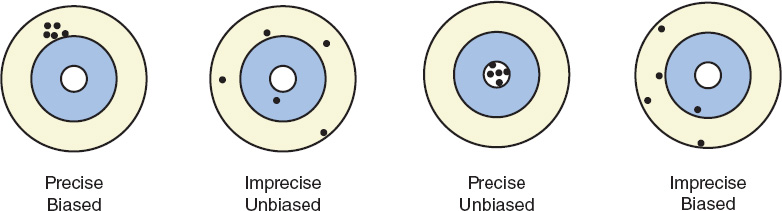
\includegraphics[width=\linewidth,trim=0 26 0 0,clip]{assets/ch04_accuracy_targets.jpeg}
\begin{tabularx}{\linewidth}{*{4}{>{\centering\arraybackslash}X}}
精密、有偏倚 & 不精密、无偏倚 & 精密、无偏倚 & 不精密、有偏倚
\end{tabularx}
\caption*{\textbf{图 4.2}\quad 不精密与偏倚的区别。}
\end{figure}\par
与精密度不同，准确度会受偏倚即系统误差影响；误差越大，变量越不准确。前述三类随机误差来源，在这里都有对应偏倚。
\begin{itemize}
\item \term{观察者偏倚}（observer bias）是观察者在感知或报告测量时，有意或无意地造成歪曲，也可能表现为系统性的仪器操作错误。例如倾向把血压读数向下取整到末位为零的 mm Hg，或访谈时使用诱导问题。
\item \term{仪器偏倚}（instrument bias）可源于机械仪器故障。例如长期未校准的秤，读数可能逐渐偏低，持续低估体重。
\item \term{参与者偏倚}（participant bias）是参与者造成的测量歪曲，例如报告事件时的偏差，也称应答者偏倚或回忆偏倚。比如，相信酒精造成自己癌症的乳腺癌患者，可能夸大饮酒量。
\end{itemize}
评估准确度的最好方法，是尽可能与\term{金标准}（gold standard）比较，即采用被认为最能代表特征真实值的技术所作的参照测量。指定什么是金标准，有时很难，需要依据本领域既往研究与专家共识。
\sourcepage{89}
连续尺度的准确程度，可用参与者中待评估测量与金标准差值的均值表示。二分类测量可用灵敏度和特异度描述相对金标准的准确度（第 13 章）。类别超过两个时，可分别计算各类判断正确的百分比。

\subsection{提高准确度的策略}
主要方法包括前述提高精密度的前四项策略，以及另外三项（表 4.4）：
\begin{enumerate}
\item 测量方法标准化。
\item 培训和认证观察者。
\item 改进仪器。
\item 仪器自动化。
\item \textbf{采用不引人注意的测量。}有时可以使参与者意识不到测量正在进行，从而消除他们有意歪曲变量的可能。例如，评估在医院餐厅设置手部消毒液及手卫生海报的效果时，让观察者混在顾客中进行观察（8）。
\item \textbf{校准仪器。}许多仪器，特别是机械和电气仪器，可通过定期用金标准校准而提高准确度。
\item \textbf{盲法。}这一经典策略并不提高测量的总体准确度，却能消除对一组比另一组影响更大的差异性偏倚。双盲试验若盲法成功，参与者和观察者都不知道分配的是有效药物还是安慰剂，结局测量的任何不准确，在两组就会相同。
\end{enumerate}
\sourcepage{90}
{\small\setlength{\tabcolsep}{3pt}
\begin{longtable}{L{33mm}L{23mm}L{48mm}L{43mm}}
\caption*{\textbf{表 4.4}\quad 减少系统误差的策略：降压治疗研究举例}\\
\toprule 策略 & 系统误差来源 & 系统误差举例 & 预防方法举例\\\midrule\endfirsthead
\toprule 策略 & 系统误差来源 & 系统误差举例 & 预防方法举例\\\midrule\endhead
1. 在操作手册中规定标准测量方法 & 观察者 & 以声音开始变弱处作舒张压，读数持续偏高 & 将舒张压的操作性定义规定为声音消失处\\
 & 参与者 & 患者刚爬楼到诊室即测量，血压持续偏高 & 规定测量前在安静房间坐 5 分钟\\
2. 培训和认证观察者 & 观察者 & 不遵守手册程序，血压读数持续偏高 & 培训者重复测量，检查观察者读数准确度\\
3. 改进仪器 & 仪器 & 上臂很粗者使用标准袖带，血压读数持续偏高 & 对肥胖或肌肉发达者使用特宽袖带\\
4. 仪器自动化 & 观察者 & 有意或无意地把随机分到有效药物组者的血压读低 & 使用自动血压测量设备\\
 & 参与者 & 有吸引力的技术人员靠近，导致血压升高 & 使用自动血压测量设备\\
\sourcepage{91}5. 不引人注意的测量 & 参与者 & 倾向高报研究药物依从性 & 测量尿中研究药物水平\\
6. 校准仪器 & 仪器 & 压力计失调，血压读数持续偏高 & 每月校准\\
7. 盲法 & 观察者 & 有意或无意地把有效治疗组血压读低 & 使用双盲安慰剂，隐瞒组别分配\\
 & 参与者 & 知道自己服有效药，倾向多报副作用 & 使用双盲安慰剂，隐瞒组别分配\\\bottomrule
\end{longtable}}
与精密度一样，针对每项测量把这七种策略实施到何种程度，取决于研究者判断。应考虑预期不准确对结论的潜在影响，以及策略的可行性和费用。前两项（标准化与培训）始终应采用；凡仪器可能随时间变化，都需要校准；只要可行，盲法就不可缺少。

\section{效度}
\term{效度}（validity）类似准确度，但在我们看来，它为衡量测量代表所关注现象的程度增添了定性层面。例如，肌酐和胱抑素 C 都由肾脏排泄，
\sourcepage{92}
两者血中浓度可以同样准确，例如距真实浓度均不超过 1\%，但衡量肾功能时，胱抑素 C 可能更有效，因为肌酐还受肌肉量影响（9）。

效度往往无法通过金标准评价，尤其是疼痛或生活质量等主观、抽象现象。可从几个方面评价此类测量方法的效度。
\begin{description}[leftmargin=2em,labelindent=0pt,style=nextline]
\item[内容效度（content validity）]考察测量对现象各个方面的覆盖程度。例如，SF-36 包含社会、身体与情绪功能、总体健康、心理健康及身体疼痛的问题，以评估生活质量（3）。
\item[表面效度（face validity）]指测量本身看起来是否合理，例如用肌无力、疲惫感、体重下降及日常步速慢来评估衰弱（10）。
\item[构念效度（construct validity）]指测量结果与理论预期相符的程度。例如，社会孤立测量应能区分几乎没有朋友、不参加社交活动的人，与朋友很多、参加多种活动的人。
\item[预测效度（predictive validity）]指预测结局的能力，例如衰弱测量能在多大程度上预测入住长期照护机构。
\item[效标关联效度（criterion-related validity）]指新测量与其他测量的相关程度，例如测量肌肉量的新生化检查与肌力测量的相关程度。
\end{description}
测量主观和抽象现象，通常先检索文献并咨询专家，寻找适合且已验证的工具，往往是问卷。这样做可使新研究结果与既往工作可比，也可能简化并加强资助申请及发表过程。
\sourcepage{93}
缺点是原有验证过程未必充分，而且现成工具可能过时，或不最适合当前问题。

若现有工具不适合，研究者可自行开发和验证新方法。这可能是一项有趣的挑战，甚至对文献作出有价值的贡献，但通常耗时费力。可以说，实际所得结论常不如“验证”一词听起来那样确定。

\section{测量方法的其他特征}
测量应足够\term{敏感}（sensitive），能够检出研究者关心的重要差异。\footnote{第 13 章将更正式地把灵敏度和特异度定义为诊断检查的特征。此处一般含义相同：敏感性关乎发现想发现之物的能力，特异性关乎避免发现不想发现之物的能力。}所需敏感程度取决于研究问题。例如，检验治疗能否改善心功能时，测量参与者 6 分钟能走的距离，可能比自报走一个街区后的气促程度，更敏感地反映心脏表现的变化。

理想测量应有\term{特异性}（specific），只代表所关注特征。例如，用超声心动图测量心脏收缩功能，比 6 分钟步行距离更特异地反映治疗对心力衰竭的作用，因为步行距离还受肺功能及腿部肌肉易疲劳程度影响。

测量必须适合研究目标。例如，把应激作为心肌梗死先行因素的研究，在确定操作性定义之前，必须先考虑关心的是心理还是身体、急性还是慢性的应激。

测量还应在样本中产生适当的反应分布。功能状态测量，若有些人得分高、另一些低，最有用。预试验的主要目的之一，就是避免实际反应全挤在可能范围的一端，即所谓“地板效应和天花板效应”。
\sourcepage{94}
只要可能，应尽量减少测量中的主观判断。减少观察者及参与者介入、使用自动化仪器，可以提高客观性。但危险是形成视野狭窄，限制观察范围及发现意外现象的能力。除定量测量外，加入开放式问题，并允许收集主观和定性资料，可以应对这一问题。

设计时常会不断加入并非研究中心、却也可能有趣的项目。额外测量的确能回答更多问题，但应记住效率及简约的重要性。整套测量应在时间和经费可承担、参与者负担可接受的条件下，收集有用资料。收集过多信息是常见错误，会使参与者疲劳、测量团队不堪重负，并给数据管理与分析增添杂乱。结果可能是花费更多，反而更难回答主要问题。

\section{利用保存材料进行测量}
某些测量只能在接触参与者时完成，但许多可以留待日后，在保存的生物样本上进行化学、遗传或其他分析，或者利用以电子形式存档的放射学等影像（表 4.5）。
\begin{bookbox}{表 4.5\quad 可在保存材料上进行的测量举例}
\begin{tabularx}{\linewidth}{L{25mm}YY}
\toprule 测量类型 & 例子 & 保存以备日后测量的材料\\\midrule
病史 & 诊断、实验室结果、药物、手术、症状、体征；应用自然语言处理 & 电子病历\\
\sourcepage{95}生化测量 & 炎症标志物、游离 DNA 水平、微生物组构成 & 血清、血浆、尿液、粪便\\
遗传或分子检查 & 全基因组测序、DNA 甲基化 & 全血或组织样本\\
影像 & 身体组成、骨结构、用人工智能分析预测疾病或结局 & X 线片、计算机断层扫描及其他方法的影像\\\bottomrule
\end{tabularx}
\end{bookbox}
保存的一个好处是，可以只对随访中发生结局的人及部分其他人进行测量，例如采用巢式病例对照研究（第 9 章），以降低费用。保存生物样本及影像，还有利于利用研究开始后的科学进展：新的想法与测量技术出现后，可申请新资助加以应用。样本应仔细采集、迅速冷冻，并在很低温度，例如 $-70\,^{\circ}\mathrm C$，甚至 $-190\,^{\circ}\mathrm C$ 下存档，使其适于未来检测。这样就能使用日益先进的测量，例如蛋白质组学或单细胞基因表达分析。应考虑保存血浆、尿液、白细胞，或用于细菌种类定量的粪便等多种样本，为未来多样化检测作准备。同时，也应取得涵盖未来广泛潜在用途的参与者知情同意。

\section{小结}
\begin{enumerate}
\item 变量分数值与分类两类。数值变量为连续（无限尺度）或离散（例如整数的有限尺度）；分类变量为无序或有序，只有两个类别的称二分类变量。
\sourcepage{96}
\item 信息更多的变量，可提高效能或减少所需样本量，顺序为：连续变量 $>$ 离散数值变量 $>$ 有序分类变量 $>$ 无序及二分类变量。
\item 测量精密度，即重复测量的可重复性，是效能和样本量的另一个主要决定因素。观察者、参与者、仪器三方面的随机误差会降低精密度。
\item 每项研究都应以操作手册明确和标准化方法，并培训和认证观察者。其他常有用的办法包括改进仪器、自动化，以及重复测量取均值。
\item 准确度是测量接近金标准的程度。来自观察者、参与者和仪器的不精密（随机误差）及偏倚（系统误差）都会降低准确度。
\item 除重复测量外，提高精密度的所有策略均有助于减少偏倚。采用不引人注意的测量及校准仪器也可减少偏倚；组间比较时，盲法可减少差异性偏倚。
\item 效度是测量代表预定现象的程度，有时可以与金标准比较评估。抽象和主观变量没有金标准时，可考察内容、表面、结构、预测及效标关联效度。
\item 单项测量应敏感、特异、适当、客观，并产生有一定范围的数值。总体测量应覆盖充分而简约，以适中时间和费用服务于研究问题，不过度增加参与者负担。
\sourcepage{97}
\item 应考虑保存生物样本、影像及其他材料，以便日后利用新技术，也可提高巢式病例对照设计的效率。
\end{enumerate}
\begin{references}
\item Kassem Z, Burmeister C, Johnson DA, et al. Reliability of birth weight recall by parent or guardian respondents in a study of healthy adolescents. BMC Res Notes. 2018;11:878.
\item Jiang M, Zou Y, Xin Q, et al. Dose-response relationship between body mass index and risks of all-cause mortality and disability among the elderly: a systematic review and meta-analysis. Clin Nutr. 2019;38(4):1511-1523.
\item Ware JE, Gandek B Jr. Overview of the SF-36 health survey and the international quality of life assessment project. J Clin Epidemiol. 1998;51:903-912. SF-36 介绍见 \url{https://www.rand.org/health-care/surveys_tools/mos/36-item-short-form.html}
\item Bland JM, Altman DG. Measurement error and correlation coefficients. BMJ. 1996;313:41-42; also, Measurement error proportional to the mean. BMJ. 1996;313:106.
\item Newman TB, Kohn M. Evidence-Based Diagnosis: An Introduction to Clinical Epidemiology. 2nd ed. Cambridge University Press; 2020: Chapter 5, 110-143.
\item Cohen J. A coefficient of agreement for nominal scales. Educ Psychol Meas. 1960;20:37-46.
\item Kuzniewicz MW, Greene DN, Walsh EM, McCulloch CE, Newman TB. Association between laboratory calibration of a serum bilirubin assay, neonatal bilirubin levels, and phototherapy use. JAMA Pediatr. 2016;170(6):557-561.
\item Filion K, Kukanich KS, Chapman B, et al. Observation-based evaluation of hand hygiene practices and the effects of an intervention at a public hospital cafeteria. Am J Infect Control. 2011;39:464-470.
\item Peralta CA, Shlipak MG, Judd S, et al. Detection of chronic kidney disease with creatinine, cystatin C, and urine albumin-to-creatinine ratio and association with progression to end-stage renal disease and mortality. JAMA. 2011;305:1545-1552.
\item Xue QL, Tian J, Fried LP, et al. Physical frailty assessment in older women: can simplification be achieved without loss of syndrome measurement validity? Am J Epidemiol. 2016;183(11):1037-1044.
\end{references}
\sourcepage{98}
\chapterappendix{4A}{握力测量的操作性定义}
\sourcepage{99}
操作手册描述研究中所有测量的实施方法及结果记录方式。本例介绍用测力计测握力。为使不同检查者及不同参与者接受相同说明，方案提供了一段必须逐字向参与者朗读的话。
\subsection{测力计握力测量规程}
测量双手握力。调节手柄，使参与者能够舒适握持。把测力计放在右手，表盘朝向掌心。肘关节屈曲 90°，前臂平行地面。
\begin{enumerate}
\item 向参与者示范，示范时说明：“这台设备测量您的手臂和上半身力量。我们会测两侧手臂的握力。我先示范一下。把肘部弯曲成 90°，前臂与地面平行。不要让手臂碰到身体侧面。在我数到三的过程中，放低设备，同时尽最大力气握紧。手臂完全伸直后，就可以松开。”
\item 每侧手臂先练习一次；若惯用右手，就从右侧开始。第二次测试时，从表盘记录以 kg 为单位的力，精确到 0.5 kg。
\item 将表盘复位，对另一侧重复上述程序。
\end{enumerate}
手臂不得接触身体。握紧应缓慢持续，不要突然猛拉。

\sourcepage{100}
\chapterappendix{4B}{第 4 章习题：规划测量}
\begin{enumerate}
\item 将以下变量归为二分类、无序分类、有序分类、连续或离散数值变量。是否能修改其中某些变量以提高效能？如何修改？
\begin{enumerate}
\item 心脏病发作史（有／无）\item 年龄\item 教育程度（大学及以上／未达大学学历）\item 种族\item 每日饮酒杯数\item 抑郁（无、轻、中、重）\item 冠状动脉闭塞百分比\item 发色\item 肥胖（$\mathrm{BMI}\geq30$ kg/m$^2$）／非肥胖（$\mathrm{BMI}<30$ kg/m$^2$）
\end{enumerate}
\item 研究者的问题是：“6 月龄时果汁摄入是否预测 1 岁时体重？”她计划前瞻性队列研究，用婴儿秤测体重。预试验发现以下问题。它们源于不精密（随机误差）、偏倚（系统误差），还是两者？主要是观察者、参与者还是仪器变异？怎样处理？
\begin{enumerate}
\item 用于校准的 10 kg 砝码，真实重量为 10.2 kg。
\item 反复称量 10 kg 砝码，均值 $\pm$ 标准差为 $10.01\pm0.2$ kg。
\item 一些婴儿害怕，扭动着想离开秤，观察者必须扶住才能完成测量。
\item 对不肯躺好的婴儿，秤指针剧烈上下摆动。
\item 有的婴儿检查前刚吃饱，有的饿着；有的称重时穿着湿尿布。
\end{enumerate}
\item 研究者想考察限制住院医师工时的影响，关注外科住院医师的职业倦怠。她计划从一份较长问卷中取两个问题，均以七级尺度作答：
\sourcepage{101}
（a）“您多常因工作感到身心耗竭？”（b）“您多常觉得，自开始住院医师培训以来，自己对人变得更冷漠？”她准备评估两题测量倦怠的效度。指出以下各项评估了何种效度：
\begin{enumerate}
\item 倦怠评分较高的住院医师，随后一年更容易退出培训。
\item 请一小组住院医师审阅后，他们认为这些问题用来了解倦怠很合理。
\item 最辛苦的轮转期间评分上升，休假期间下降。
\item 一项涉及一万多名医学生、住院医师及执业医师的既往研究显示，两题几乎完整覆盖了广泛接受、但长得多的 Maslach 倦怠量表中情绪耗竭与人格解体两个维度（1）。
\end{enumerate}
\end{enumerate}
\begin{references}
\item West CP, Dyrbye LN, Sloan JA, Shanafelt TD. Single item measures of emotional exhaustion and depersonalization are useful for assessing burnout in medical professionals. J Gen Intern Med. 2009;24(12):1318-1321.
\end{references}
